


\tikzset{every picture/.style={line width=0.75pt}} %set default line width to 0.75pt        

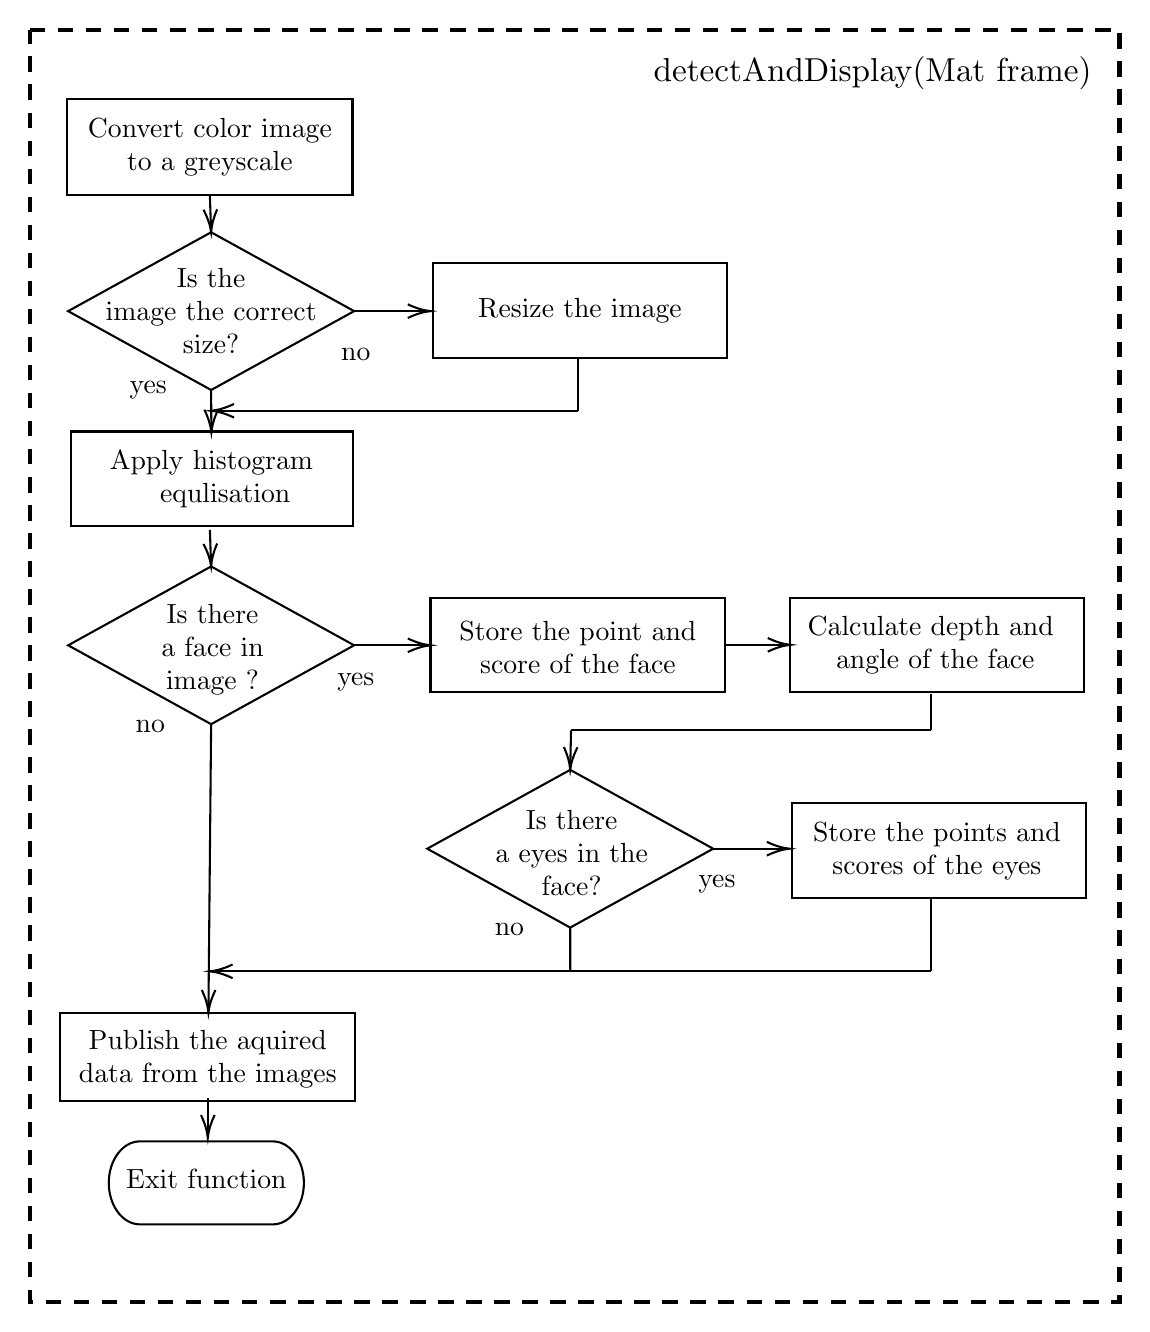
\begin{tikzpicture}[x=0.75pt,y=0.75pt,yscale=-1,xscale=1]
%uncomment if require: \path (0,633.0166625976562); %set diagram left start at 0, and has height of 633.0166625976562

%Flowchart: Terminator [id:dp5529482487941668] 
\draw   (71.04,539) -- (134.96,539) .. controls (143.27,539) and (150,547.95) .. (150,559) .. controls (150,570.05) and (143.27,579) .. (134.96,579) -- (71.04,579) .. controls (62.73,579) and (56,570.05) .. (56,559) .. controls (56,547.95) and (62.73,539) .. (71.04,539) -- cycle ;
%Flowchart: Process [id:dp44317618562586525] 
\draw   (36,37) -- (173.42,37) -- (173.42,83) -- (36,83) -- cycle ;
%Flowchart: Decision [id:dp20710004786998082] 
\draw   (105.31,101) -- (174.21,139) -- (105.31,177) -- (36.42,139) -- cycle ;
%Straight Lines [id:da4728288029376392] 
\draw    (173,139) -- (209,139) ;
\draw [shift={(211,139)}, rotate = 180] [color={rgb, 255:red, 0; green, 0; blue, 0 }  ][line width=0.75]    (10.93,-3.29) .. controls (6.95,-1.4) and (3.31,-0.3) .. (0,0) .. controls (3.31,0.3) and (6.95,1.4) .. (10.93,3.29)   ;

%Straight Lines [id:da28089317347513165] 
\draw    (282,162.03) -- (282,187) ;


%Straight Lines [id:da3618479498651064] 
\draw    (282,187) -- (107.42,187) ;
\draw [shift={(105.42,187)}, rotate = 360] [color={rgb, 255:red, 0; green, 0; blue, 0 }  ][line width=0.75]    (10.93,-3.29) .. controls (6.95,-1.4) and (3.31,-0.3) .. (0,0) .. controls (3.31,0.3) and (6.95,1.4) .. (10.93,3.29)   ;

%Flowchart: Process [id:dp3971262056258782] 
\draw   (37.71,197) -- (173.71,197) -- (173.71,242.53) -- (37.71,242.53) -- cycle ;
%Flowchart: Decision [id:dp5544530698534428] 
\draw   (105.31,262) -- (174.21,300) -- (105.31,338) -- (36.42,300) -- cycle ;
%Straight Lines [id:da11849876539933246] 
\draw    (173,300) -- (209,300) ;
\draw [shift={(211,300)}, rotate = 180] [color={rgb, 255:red, 0; green, 0; blue, 0 }  ][line width=0.75]    (10.93,-3.29) .. controls (6.95,-1.4) and (3.31,-0.3) .. (0,0) .. controls (3.31,0.3) and (6.95,1.4) .. (10.93,3.29)   ;

%Flowchart: Process [id:dp8189382759950868] 
\draw   (384,277) -- (526,277) -- (526,322.53) -- (384,322.53) -- cycle ;
%Straight Lines [id:da38367274179586863] 
\draw    (104.71,83.43) -- (105.24,99) ;
\draw [shift={(105.31,101)}, rotate = 268.03] [color={rgb, 255:red, 0; green, 0; blue, 0 }  ][line width=0.75]    (10.93,-3.29) .. controls (6.95,-1.4) and (3.31,-0.3) .. (0,0) .. controls (3.31,0.3) and (6.95,1.4) .. (10.93,3.29)   ;

%Straight Lines [id:da4076173099306175] 
\draw    (105.31,177) -- (105.41,195.43) ;
\draw [shift={(105.42,197.43)}, rotate = 269.71] [color={rgb, 255:red, 0; green, 0; blue, 0 }  ][line width=0.75]    (10.93,-3.29) .. controls (6.95,-1.4) and (3.31,-0.3) .. (0,0) .. controls (3.31,0.3) and (6.95,1.4) .. (10.93,3.29)   ;

%Straight Lines [id:da7923134197816337] 
\draw    (104.71,244.43) -- (105.24,260) ;
\draw [shift={(105.31,262)}, rotate = 268.03] [color={rgb, 255:red, 0; green, 0; blue, 0 }  ][line width=0.75]    (10.93,-3.29) .. controls (6.95,-1.4) and (3.31,-0.3) .. (0,0) .. controls (3.31,0.3) and (6.95,1.4) .. (10.93,3.29)   ;

%Flowchart: Process [id:dp06214403298597504] 
\draw   (211,277) -- (353,277) -- (353,322.53) -- (211,322.53) -- cycle ;
%Straight Lines [id:da09540214320175266] 
\draw    (353.42,299.77) -- (382.42,299.77) ;
\draw [shift={(384.42,299.77)}, rotate = 180] [color={rgb, 255:red, 0; green, 0; blue, 0 }  ][line width=0.75]    (10.93,-3.29) .. controls (6.95,-1.4) and (3.31,-0.3) .. (0,0) .. controls (3.31,0.3) and (6.95,1.4) .. (10.93,3.29)   ;

%Straight Lines [id:da04226589467849684] 
\draw    (452,323.43) -- (452,341) ;


%Straight Lines [id:da29543893735919613] 
\draw    (452,341) -- (278.71,341) ;


%Flowchart: Decision [id:dp44558589780986957] 
\draw   (278.31,360) -- (347.21,398) -- (278.31,436) -- (209.42,398) -- cycle ;
%Straight Lines [id:da24851075892837005] 
\draw    (346,398) -- (382,398) ;
\draw [shift={(384,398)}, rotate = 180] [color={rgb, 255:red, 0; green, 0; blue, 0 }  ][line width=0.75]    (10.93,-3.29) .. controls (6.95,-1.4) and (3.31,-0.3) .. (0,0) .. controls (3.31,0.3) and (6.95,1.4) .. (10.93,3.29)   ;

%Straight Lines [id:da28050138620141496] 
\draw    (278.71,341) -- (278.35,358) ;
\draw [shift={(278.31,360)}, rotate = 271.19] [color={rgb, 255:red, 0; green, 0; blue, 0 }  ][line width=0.75]    (10.93,-3.29) .. controls (6.95,-1.4) and (3.31,-0.3) .. (0,0) .. controls (3.31,0.3) and (6.95,1.4) .. (10.93,3.29)   ;

%Flowchart: Process [id:dp21374462121931614] 
\draw   (385,376) -- (527,376) -- (527,421.53) -- (385,421.53) -- cycle ;
%Flowchart: Process [id:dp20952810314397752] 
\draw   (212,116) -- (354,116) -- (354,161.53) -- (212,161.53) -- cycle ;
%Straight Lines [id:da015454942041956077] 
\draw    (452,457.08) -- (106.71,457.08) ;
\draw [shift={(104.71,457.08)}, rotate = 360] [color={rgb, 255:red, 0; green, 0; blue, 0 }  ][line width=0.75]    (10.93,-3.29) .. controls (6.95,-1.4) and (3.31,-0.3) .. (0,0) .. controls (3.31,0.3) and (6.95,1.4) .. (10.93,3.29)   ;

%Straight Lines [id:da31054275104310947] 
\draw    (452,421.42) -- (452,457.08) ;


%Straight Lines [id:da7440000994161402] 
\draw    (278.31,436) -- (278.35,457.08) ;


%Straight Lines [id:da18463267912095405] 
\draw    (105.31,338) -- (104.02,475) ;
\draw [shift={(104,477)}, rotate = 270.54] [color={rgb, 255:red, 0; green, 0; blue, 0 }  ][line width=0.75]    (10.93,-3.29) .. controls (6.95,-1.4) and (3.31,-0.3) .. (0,0) .. controls (3.31,0.3) and (6.95,1.4) .. (10.93,3.29)   ;

%Flowchart: Process [id:dp2312308746908307] 
\draw   (32.71,477) -- (174.71,477) -- (174.71,519.33) -- (32.71,519.33) -- cycle ;
%Straight Lines [id:da7120795123598685] 
\draw    (103.71,518.25) -- (103.71,535.25) ;
\draw [shift={(103.71,537.25)}, rotate = 270] [color={rgb, 255:red, 0; green, 0; blue, 0 }  ][line width=0.75]    (10.93,-3.29) .. controls (6.95,-1.4) and (3.31,-0.3) .. (0,0) .. controls (3.31,0.3) and (6.95,1.4) .. (10.93,3.29)   ;

%Shape: Rectangle [id:dp5474626172021357] 
\draw  [dash pattern={on 5.63pt off 4.5pt}][line width=1.5]  (17.92,3.43) -- (542.92,3.43) -- (542.92,616.42) -- (17.92,616.42) -- cycle ;

% Text Node
\draw (103,557) node  [align=left] {Exit function};
% Text Node
\draw (104.71,60) node  [align=center] {Convert color image\\to a greyscale};
% Text Node
\draw (283,138.77) node  [align=center] {Resize the image};
% Text Node
\draw (175,160) node  [align=left] {no};
% Text Node
\draw (105.31,139) node  [align=center] {	Is the \\image the correct \\	 size?};
% Text Node
\draw (105.42,219.77) node  [align=center] {Apply histogram\\ \ \ \ equlisation };
% Text Node
\draw (282,301) node  [align=center] {Store the point and\\score of the face};
% Text Node
\draw (175,318) node  [align=left] {yes};
% Text Node
\draw (106,302) node  [align=center] { Is there \\a face in \\ image ?};
% Text Node
\draw (452,299.77) node  [align=center] {Calculate depth and\\ \ angle of the face};
% Text Node
\draw (75,177) node  [align=left] {yes};
% Text Node
\draw (76,339) node  [align=left] {no};
% Text Node
\draw (455,399) node  [align=center] {Store the points and\\scores of the eyes};
% Text Node
\draw (349,415) node  [align=left] {yes};
% Text Node
\draw (279,400) node  [align=center] {Is there \\a eyes in the\\ face?};
% Text Node
\draw (249,437) node  [align=left] {no};
% Text Node
\draw (103.71,499.45) node  [align=center] { Publish the aquired\\data from the images};
% Text Node
\draw (424,24.55) node [scale=1.2] [align=left] {detectAndDisplay(Mat frame)};


\end{tikzpicture}

